\documentclass{beamer}
\usetheme{Boadilla}
\usepackage{hyperref}
\usepackage{graphicx}
\usepackage{fancyvrb}
\usepackage{multicol}
\usepackage{adjustbox}
\usepackage{tikz}
\usetikzlibrary{shapes,positioning}
\newcommand{\foo}{\hspace{-2.3pt}$\bullet$ \hspace{5pt}}
\usepackage{subfig}
\usepackage[backend=biber,authordate]{biblatex-chicago}
\addbibresource{citations.bib}
\usepackage{pgfpages}
\usepackage{xcolor}
\definecolor{ao(english)}{rgb}{0.0, 0.5, 0.0}
\definecolor{burgundy}{rgb}{0.5, 0.0, 0.13}
%\setbeameroption{show notes}
\setbeameroption{show notes on second screen=right}
%\setbeameroption{hide notes}

\title{Dynamic Programming for Beat Tracking}
\author{Sevag Hanssian}
\date{Feburary 16, 2021}
\institute{MUMT 621, Winter 2021}
\setbeamertemplate{navigation symbols}{}

\begin{document}

\begin{frame}
\maketitle
\end{frame}

\begin{frame}
	\frametitle{Dynamic programming}
	\vspace{0.5em}
	\includegraphics[height=1.5cm]{./clrs.jpg}\footfullcite{clrs} 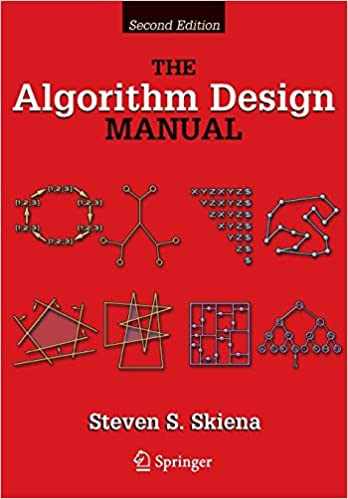
\includegraphics[height=1.5cm]{./skiena.jpg}\footfullcite{skiena}\\
	Dynamic programming applies to optimization problems in which a set of choices must be made in order to arrive at an optimal solution -- we seek to find a solution that \textbf{maximizes or minimizes some function}.\\
	\vspace{1em}
	Greedy algorithms make the best local choice -- efficient but doesn't guarantee a globally optimal solution. Exhaustive search algorithms try all combinations of choices, at a \textbf{prohibitive cost in time complexity}.\\
	\vspace{1em}
	As choices are made, \textbf{subproblems} of the same form arise, often more than once. Dynamic programming's \textbf{key technique is to store solutions to each subproblem} while searching all possibilities.
\end{frame}

\begin{frame}[fragile]
	\frametitle{Time complexity and Big-Oh notation}
	Algorithms in computer science are often described by their time complexity in a hypothetical computer where\footcite{skiena} \textbf{simple operations take 1 time step}. Big-Oh provides the upper bound of algorithm running time in relation to number of input elements.
	\begin{verbatim}
	function linearSearch(animalToFind, arrayOfAnimals) -> bool
	    for every animal in arrayOfAnimals
	        if animal == animalToFind
	            return true
	    return false
	\end{verbatim}
	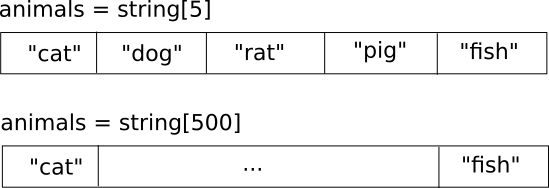
\includegraphics[width=5cm]{./linearsearch.png}\\
	Linear search is $O(n)$ -- directly proportional to input size
\end{frame}

\note{
	\begin{itemize}
		\item
			Suppose an algorithm written in C is two times faster than the same algorithm written in Java -- doesn't tell us much about the algorithm at all

		\item
			Ignores specific implementation details such as: programming languages, CPU models, types of storage -- the goal is to understand and study algorithms in a language- and machine-independent manner. Details are less important than the worst-case time complexity
	\end{itemize}
}

\begin{frame}
	\frametitle{Common values for Big-Oh}
	\begin{figure}
		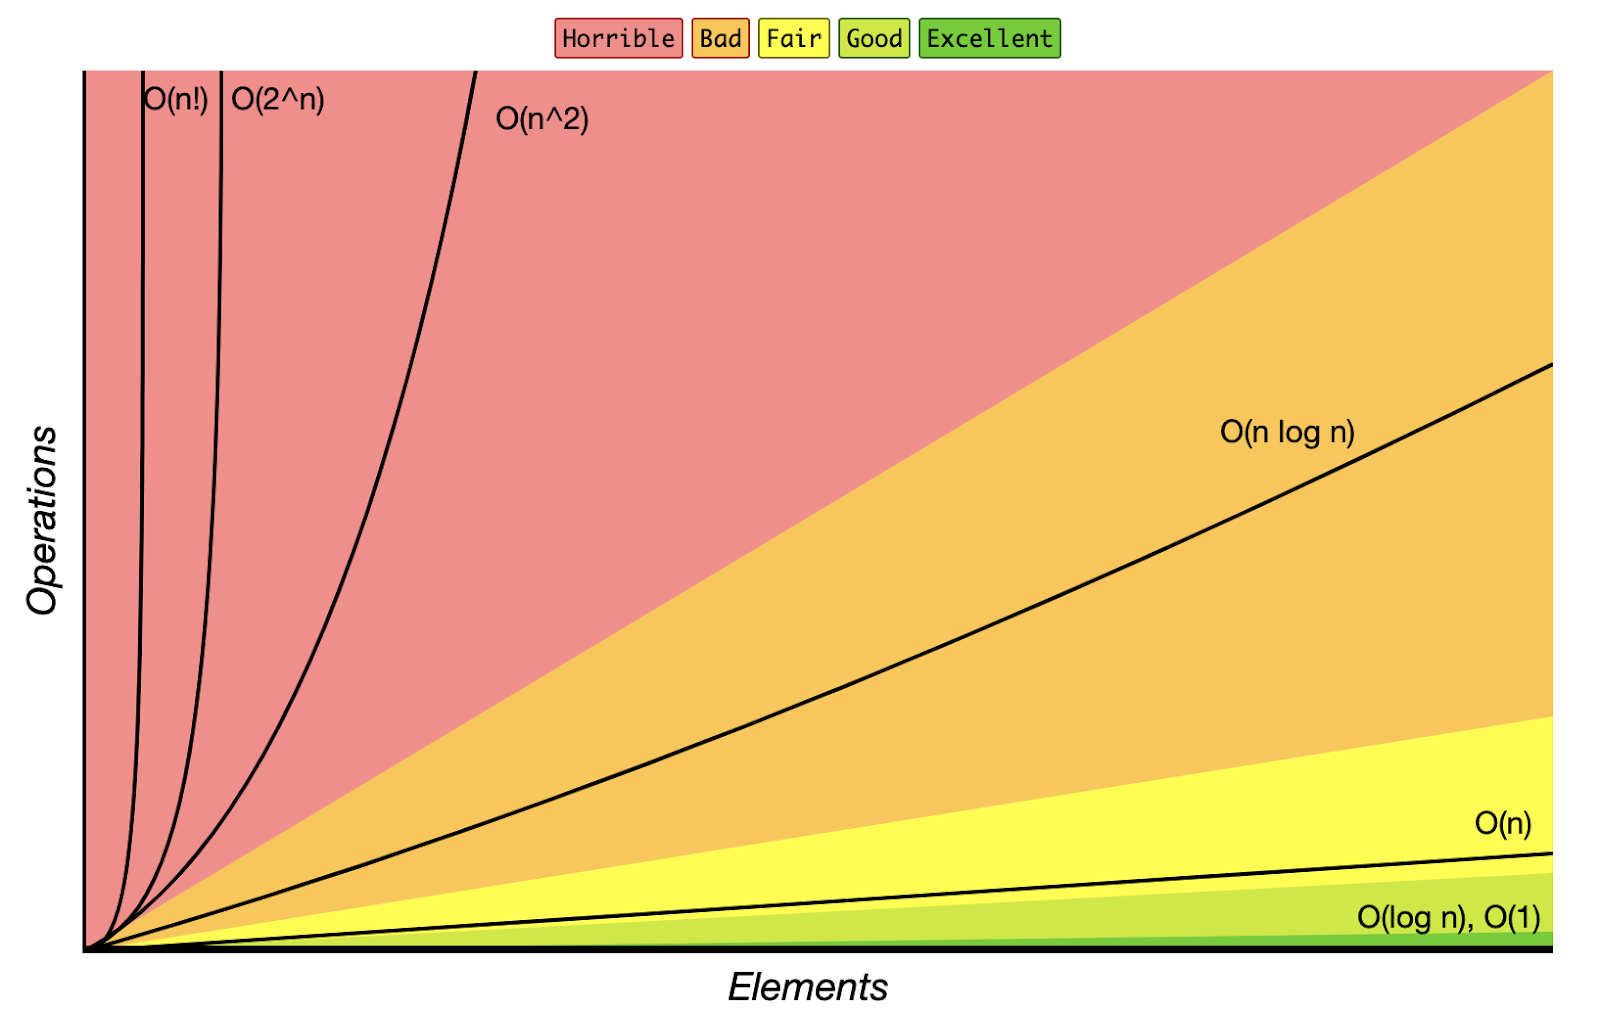
\includegraphics[width=8cm]{./bigo.png}
		\caption{Big-Oh complexity chart\footfullcite{dzone}}
	\end{figure}
	Analogous concept: space complexity
\end{frame}

\begin{frame}
	\frametitle{Recursion}
	Many algorithms are recursive in structure -- to solve a problem, they call themselves recursively to deal with closely related \textbf{subproblems}\footcite{clrs}\\
	\vspace{1em}
	Typical paradigm is \textbf{divide-and-conquer}:
	\begin{enumerate}
		\item
			\textbf{Divide} the problem into a number of subproblems
		\item
			\textbf{Conquer} the subproblems by solving them recursively -- if the subproblem is ``small enough,'' just solve it in a straightforward manner
		\item
			\textbf{Combine} the solutions to the subproblems into a solution for the original problem
	\end{enumerate}
\end{frame}

\begin{frame}[fragile]
	\frametitle{Recursion example -- Fibonacci sequence}
	The Fibonacci sequence: 0, 1, 1, 2, 3, 5, 8, 13, ...\footcite{clrs}
	\vspace{1em}
	\begin{columns}
		\begin{column}{0.45\textwidth}
		Recursive definition:
		\begin{enumerate}
			\item
				$f_{0} = 0$
			\item
				$f_{1} = 1$
			\item
				$f_{n} = f_{n-1} + f_{n-2} \text{ for } n \ge 2$
		\end{enumerate}
		\begin{verbatim}
		function fib(n int) -> int {
		    if n <= 1 {
			return n
		    }
		    return fib(n-1) + fib(n-2)
		}
		\end{verbatim}
		\end{column}
		\begin{column}{0.45\textwidth}
		What happens when we call fib(5)
		\begin{figure}
			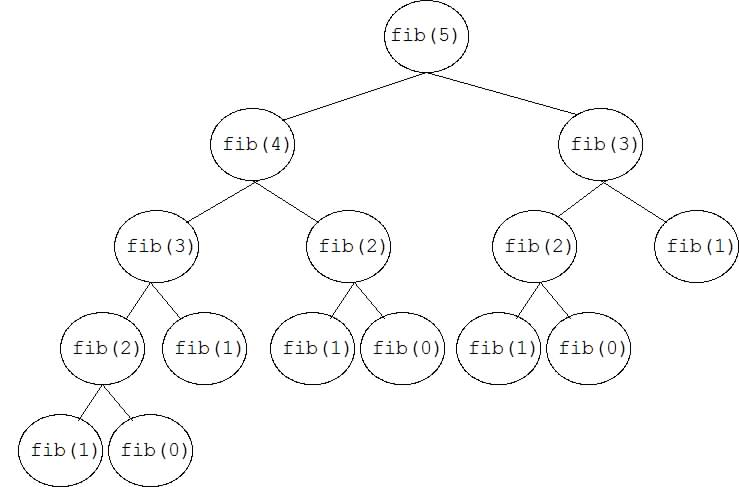
\includegraphics[width=5.25cm]{./fibrecurse.jpg}\footnotemark
		\end{figure}
		\end{column}
	\end{columns}
\footnotetext{\fullcite{fibrecurse}}
\end{frame}

\begin{frame}[fragile]
	\frametitle{Fibonacci sequence with dynamic programming}
	Trade off space for time by storing the computed subproblems:
	\begin{verbatim}
	int[10000] cache; // global storage array

	function init_fib() {
	    cache[0] = 0;
	    cache[1] = 1;
	    for i = 2; i < 10000; i++ {
	        cache[i] = -1;
	    }
	}
	function fib(n int) -> int {
	    if cache[n] == -1 {
        cache[n] = fib(n-1) + fib(n-2);
	    }
	    return cache[n];
	}
	\end{verbatim}
\end{frame}

\note{
	\begin{itemize}
		\item
			No optimizing here -- simply caching a recursive function gets you, most of the way to the benefits of dynamic programming
		\item
			Labmate Nestor got an improvement of 34\% by caching partial results in a Python piece of music code doing something with chord keys and voicings and mus21
	\end{itemize}
}

\begin{frame}
	\frametitle{Beat tracking as an optimization problem}
	Beat tracking as an optimization problem\footfullcite{ellis}: $C(\{t_{i}\}) = \sum_{i=1}^{N}O(t_{i}) + \alpha\sum_{i=2}^{N}F(t_{i}-t_{i-1}, \tau_{p})$\\
	\vspace{1em}
	\begin{itemize}
		\item
			Compute an onset strength envelope $O(t)$ for the whole signal
		\item
			Compute a target tempo by applying autocorrelation (including some human tempo preference) to find periodicity in the onsets
		\item
			Optimize the score $C(t_{i})$ of a beat at time $t_{i}$ based on two terms:
			\begin{enumerate}
				\item
					$O(t_{i})$ -- the onset strength envelope should be strong at tentative beat location $t_{i}$
				\item
					$F(t_{i}-t_{i-1}, \tau_{p})$ or $F(\Delta t, \tau_{p})$ -- there should be consistency between the inter-beat interval $\Delta t$ and the beat spacing $\tau_{p}$ from target tempo
			\end{enumerate}
			$\alpha$ is the weighting term to balance the importance of the 2 terms
	\end{itemize}
	Exponential search over all time $t_{i}$\footfullcite{ellis2}
\end{frame}

\note{
	\begin{itemize}
		\item
			in the paper he says 120bpm is a natural choice for listeners
		\item
			Exhaustive search algorithms try all combinations of choices, at a \textbf{prohibitive cost in time complexity}
	\end{itemize}
}

\begin{frame}
	\frametitle{Onset strength envelope and tempo estimation}
	Onsets mark the start of a musical note or acoustic event\footfullcite{onsets}
	\begin{figure}
		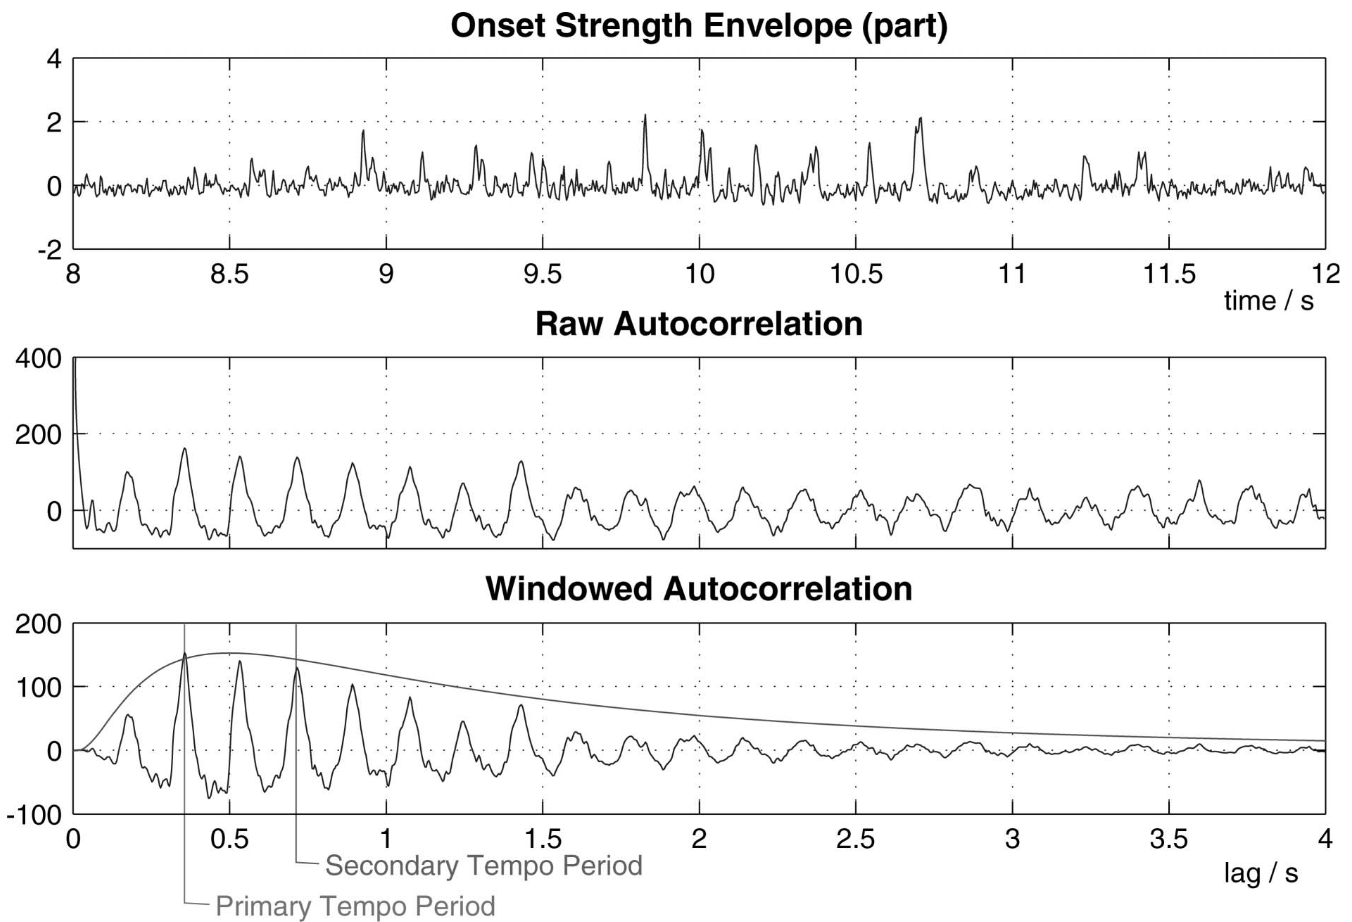
\includegraphics[height=4cm]{./onset2.png}
		\caption{Top: onset strength envelope. Middle: raw autocorrelation. Bottom: autocorrelation with perceptual weighting window.\footcite{ellis}}
	\end{figure}
\end{frame}

\note{
	\begin{itemize}
		\item
			Human tempo perception is known to have a bias towards 120 BPM. We apply a perceptual weighting window to the raw autocorrelation to downweight periodicity peaks far from this bias
		\item
			This graph contains all the information you need for a beat tracker! but remember the optimization goals
	\end{itemize}
}

\begin{frame}
	\frametitle{Beat tracking with dynamic programming}
	Recall: beat tracking as an optimization problem\footcite{ellis}:
	\[ C(\{t_{i}\}) = \sum_{i=1}^{N}O(t_{i}) + \alpha\sum_{i=2}^{N}F(t_{i}-t_{i-1}, \tau_{p}) \]
	Recursive definition from best possible score $C^{*}(t)$ at time $t$:
	\[ C^{*}(t) = O(t) + \text{max}_{\tau = 0...t}\{\alpha F(t-\tau, \tau_{p}) + C^{*}(\tau)\} \]
	Record preceding beat time that gave best score:
	\[ P^{*}(t) = \text{argmax}_{\tau = 0...t} \{\alpha F(t-\tau, \tau_{p}) + C^{*}(\tau)\} \]
\end{frame}

\begin{frame}
	\frametitle{Penalty term}
	Function $F$ is a squared-error applied to the log-ratio of actual to ideal time spacing:
	\[ F(\Delta t, \tau) = -\Big(\log\frac{\Delta t}{\tau}\Big)^{2} \]
	In practice, only need to search a limited range of $\tau$ since the penalty term $F$ grows the further you are from $\tau_{p}$ -- search in $\tau = t - 2\tau_{p} ... t - \frac{\tau_{p}}{2}$
	\begin{figure}
		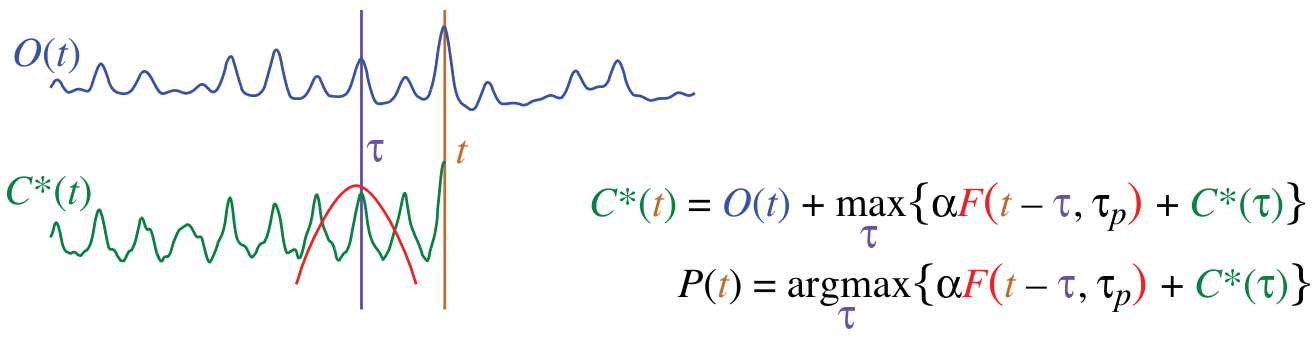
\includegraphics[width=11cm]{./ellisdp.png}
		\caption{Beat tracking by dynamic programming\footcite{ellis2}}
	\end{figure}
\end{frame}

\end{document}
